\chapter{电场}

\begin{introduction}
	\item \nameref{7.1}
	\item \nameref{7.2}
	\item \nameref{7.3}
	\item \nameref{7.4}
	\item \nameref{7.5}
\end{introduction}

电荷运动时同时激发电场与磁场, 相互联系, 较难研究, 本章在电荷静止的条件下研究其激发的电场. 正像研究牛顿定律离不开刚体, 质点, 速度, 加速度, 研究电场也离不开电荷量, 导体, 库仑定律, 场强等模型或物理量. 

\section{与电场有关的概念}\label{7.1}

\begin{definition}[电荷量]
	电中性物体得失正负电荷时会成为带电体, 其显露的电荷数为其电荷量. 
\end{definition}

\begin{axiom}[电荷守恒]
	宏观过程中, 一种电荷消失或出现, 一定有等量异种电荷消失或出现. 
	
	此时电荷守恒表述为: 电荷既不能被创造也不能被消灭, 只能从一部分转移到另一部分. 微观过程中, 电子可以由“无”到“有”, 从“有”至“无”, 如光子与原子核作用有
	
	\begin{align*}
		&r \rightarrow e^{+} + e^{-} \quad \text{(电子创生)} \\
		&e^{+} + e^{-} \rightarrow r \quad \text{(电子湮没)}
	\end{align*}
	
	但系统总电荷守恒. 
	
	因此无论宏观微观电荷守恒可表述为系统总电荷守恒, 在计算静平衡时可作为一个方程式用. 
\end{axiom}

\begin{axiom}[库仑定律]
	真空中, 两个静止点电荷之间的作用力$\va*{F}_{12}(\va*{F}_{21})$满足: 
	
	\begin{equation}
		\abs{\va*{F}_{12}} = k \dfrac{q_1 q_2}{r^2} \label{C7-eq1}
	\end{equation}
	
	方向沿两点电荷连线, 同性相斥, 异性相吸. 
	
	\vskip 0.2cm
	
	其中, $k = \dfrac{1}{4\pi \varepsilon_0}$, 为了后续推导方便, 注意用$\dfrac{1}{4\pi \varepsilon_0}$代替$k$, 戒除高中的习惯. 
	
\end{axiom}

\begin{figure}[H]
	\centering
	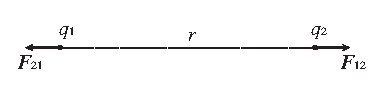
\includegraphics[scale=1.0]{C7-fig1.eps}
	\caption{两点电荷间的作用}
	\label{C7-fig1}
\end{figure}

\begin{note}
	
	$\bullet$ 点电荷为理想模型, 当两带电体自身线度与之间距离相比可忽略时可自然等效. 
	
	$\bullet$ 真空中$\varepsilon=\varepsilon_0$, 而在均匀介质中$\varepsilon=\varepsilon_0\varepsilon_r$, 代入公式时要注意($\varepsilon_0$为真空中介电常数, $\varepsilon$为某均匀同性介质中的介电常数, $\varepsilon_r$则为该介质的相对介电常数, 无单位). 
	
	$\bullet$ 若有许多点电荷, 则任一点电荷所受库仑力为其他点电荷的力的矢量和. 
	
\end{note}

\begin{definition}[电场]
	万有引力不是一种接触力, 两块磁石之间不用接触也可有里的作用, 力如何传递呢? 因为超距作用被否认了, 所以提出了场. 力由场传递, 而场由带电体激发, 静电场是相对观察者静止的电荷激发出的电场. 场是一种物质, 电荷激发出了这种物质, 电荷在场中受场的力, 运动时还会接受场做的功, 为了描述场(就像描述宏观物体所提出质量, 速度一样)提出场的强度(重力加速度就可以理解为重力场的场强). 
\end{definition}

\begin{definition}[电场强度]
	
	\begin{equation}
		\va*{E} = \dfrac{\va*{F}}{q_0} \label{C7-eq2}
	\end{equation}
	
	电场强度是电场本身的性质, 与电场中是否存在实验电荷无关. 就像一个六十公斤的人无论是否去称体重均为六十公斤一样. 
	
	$\bullet$ 特别地, 点电荷场强由$q_1$激发
	
	\begin{equation}
		E = \dfrac{q_1}{4 \pi \varepsilon_0 r^2} \label{C7-eq3}
	\end{equation}
	
	$\bullet$ 点电荷系场强由点电荷$\va*{E}$矢量叠加得到. 
	
	$\bullet$ 连续带电体场强, 取微元, 对任一微元列出场强表达式, 再进行矢量积分即可(把矢量分解成$\va*{x}$, $\va*{y}$方向的分量后与一维线积分一样, 偶尔可用矢量对称性简化过程). 
	
\end{definition}

下面对几种常见连续带电体进行求解. 

\vskip 0.3cm

\begin{example}
	有限长均匀带电细棒, 电荷线密度为$\lambda$, 求距棒$a$处一点$P$的场强.
	
	\begin{figure}[H]
		\centering
		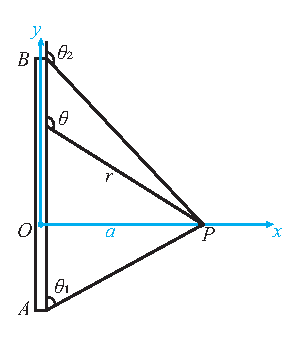
\includegraphics[scale=1.0]{C7-fig2.eps}
		\caption{有限长均匀带电细棒}
		\label{C7-fig2}
	\end{figure}
	
	\begin{solution}
		假设细棒带正电, 带负电可把$\lambda$变为负值代入以调整方向. 
		
		由点电荷的场强公式有
		
		\begin{equation*}
			\begin{cases}
				E = \dfrac{1}{4\pi \varepsilon_0} \dfrac{\lambda \dd{y}}{r^2} \\
				r \sin \theta = a 
			\end{cases}
		\end{equation*}
		
		于是
		
		\begin{align*}
			E &= \dfrac{\sin^2 \theta}{4\pi \varepsilon_0} \dfrac{\lambda \dd{y}}{a^2} \\
			E_x &= \dfrac{\sin^3 \theta}{4\pi \varepsilon_0} \dfrac{\lambda \dd{y}}{a^2} \\
			E_y &= \dfrac{\sin \theta \cos \theta}{4\pi \varepsilon_0} \dfrac{\lambda \dd{y}}{a^2} 
		\end{align*}
		
		又\footnote{这里微元为$\dd{y}$, 但明显要对$\theta$进行积分, 所以要找$\dd{y}$与$\theta$的关系, 这种变换积分未知量的操作在日后习题考试中常有. }
		
		\begin{equation*}
			- \dfrac{a}{\tan \theta} = y ~\Rightarrow~ \dd{y} = a \csc^2 \theta \dd{\theta}
		\end{equation*}
		
		如此便得到
		
		\begin{align*}
			E_x &= \int_{\theta_1}^{\theta_2} \dfrac{\lambda}{4 \pi \varepsilon_0 a} \sin \theta \dd{\theta} = \dfrac{\lambda}{4 \pi \varepsilon_0 a} (\cos \theta_1 - \cos \theta_2) \\
			E_y &= \int_{\theta_1}^{\theta_2} \dfrac{\lambda}{4 \pi \varepsilon_0 a} \cos \theta \dd{\theta} = \dfrac{\lambda}{4 \pi \varepsilon_0 a} (\sin \theta_2 - \sin \theta_1)
		\end{align*}
		
	\end{solution}
	 
\end{example}

\begin{note}
	
	\indent 首先要记住$\dfrac{\lambda}{4\pi \varepsilon_0}$, 然后记住$E_x$与$\cos \theta$有关, $E_y$与$\sin \theta$有关. $\cos \theta_1$, $\cos \theta_2$的正负决定$E_x$是从棒指向$P$点还是从$P$点指向棒. 如果棒带正电自然为前者, 反之把$\lambda$换成负的即可(但形式不变, 所以可以统一用正电记). $y$方向就看$P$点离哪一端近, 这样哪一边的$y$方向合场强小, 电场就向哪一边, 如下图所示. 
	
	\begin{figure}[h]
		\centering
		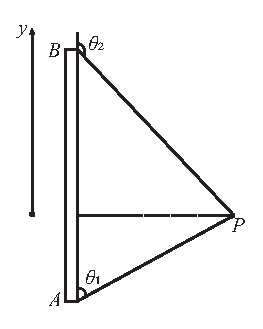
\includegraphics[scale=0.8]{C7-fig3.eps}
		\label{C7-fig3}
	\end{figure}
	
	均匀带电的话两端的$l$的$y$方向的场强相抵, 则$P$点在$y$方向上的场强向下, 大小为$E_y = \dfrac{\lambda (\sin \theta_2 - \sin \theta_1)}{4 \pi \varepsilon_0 a}$. 
	
\end{note}

\vskip 0.3cm

\begin{example}
	无限长均匀带点棒, 此时认为$\theta_1=0$, $\theta_2=\pi$, $P$点无论在何处, 均相当于中点位置, 于是$E_y=0$, $E_x$由前推导知为$\dfrac{\lambda}{2 \pi \varepsilon_0 a}$. 
\end{example}

\vskip 0.3cm

\begin{example}
	对于均匀带电细圆环轴线上的场强分布, 首先就要想到除$x$方向外所有场强均相互抵消为0, 故合场强沿$x$方向, 取一小段$r\dd{\theta}\lambda$, 则其在$P$点$x$方向场强为
	\begin{align*}
		\dd{E_x} &= \dfrac{1}{4\pi\varepsilon_0} \dfrac{r\dd{\theta}\lambda}{a^2+r^2}\cos\varphi \\
		\cos \varphi &= \dfrac{a}{\sqrt{a^2+r^2}}
	\end{align*}
    
    \begin{figure}[h]
    	\centering
    	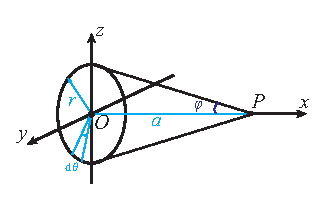
\includegraphics[scale=1.4]{C7-fig4.eps}
    	\caption{均匀带电细圆环}
    \end{figure}
    
    对$\theta$从0到$2\pi$积分即可得
	
	\begin{equation*}
		E_x=\dfrac{Qa}{4\pi\varepsilon_0{(a^2+r^2)}^{{\frac{3}{2}}}}
	\end{equation*}
    
    其中$Q=2\pi r\lambda$为总电量, 不用$\lambda$表示是为了方便下面的推导. 
	
\end{example}

\vskip 0.3cm

\begin{example}
	内外半径分别为$R_1$, $R_2$的圆环形平面均匀带电, 带电量$Q$, 轴线上的任一点的场强. 圆环形可以当作由无数细圆环拼成, 我们取一半径为$r$, 宽为$\dd{r}$的细圆环, 电荷面密度
	
	\begin{equation*}
		\sigma = \dfrac{Q}{\pi R_2^2 - \pi R_1^2}
	\end{equation*}
	
	\begin{figure}[h]
		\centering
		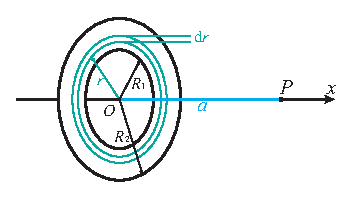
\includegraphics[scale=1.3]{C7-fig5.eps}
		\caption{均匀带电圆环平面}
	\end{figure}
	
	细圆环电量为$2\pi r_1 \sigma \dd{r}$, 由上例知这一个半径$r_1$的细圆环产生的电场强度为
	
	\begin{align*}
		E_0 &= \dfrac{Q_1 a}{4 \pi \varepsilon_0 {(a^2 + r_1^2)}^{{\frac{3}{2}}}} \\
		Q_1 &= \dfrac{2\pi r_1Q}{\pi R_2^2 - \pi R_1^2}
	\end{align*}
	
	从$R_1$到$R_2$对$\dd{r}$积分得
	
	\begin{equation*}
		E = \dfrac{\sigma x}{2 \varepsilon_0}\qty[\dfrac{1}{{(r_1^2 + x^2)}^{{\frac{1}{2}}}} - \dfrac{1}{{(r_2^2 + x^2)}^{{\frac{1}{2}}}}]
	\end{equation*}
	
\end{example}

\begin{note}
	
	$\bullet$ 如果是一个圆形平板, $R_1=0$. 
	
	$\bullet$ 如果$a\gg R_1$, $a\gg R_1$, 可看成电量为$Q$的点电荷, $E = \dfrac{Q}{4 \pi \varepsilon_0 a^2}$.
	
	$\bullet$ 若为无限大平板, $R_2 \rightarrow \infty$, $R_1=0$, $E = \dfrac{\sigma}{2\varepsilon_0}$.
	
	\vskip 0.2cm
	
	$\bullet$ 这一部分需要自己多推导几次, 防止遗忘. 
	
\end{note}

\section{描绘电场的方法} \label{7.2}

在上一节\nameref{7.1}中, 我们讨论了电场有关的物理量, 并推导了几种规则图形的场强分布, 以下要提出描绘电场的方法以及两个相关定理. 

\subsection{电场线}

用电场线描绘电场. 电场线上任一点的切线方向即为这一点场强的方向, 电场线的疏密反映出附件场强的大小. 

其实和高中课本上的没太大区别. 至于电场的提出的具体思路还是说不清, 只是知道它确实是有用即可. 

\begin{note}
	
	$\bullet$ 电场线起于正电荷或无穷远处, 终于负电荷或无穷远处. 
	
	$\bullet$ 电场线不相交, 不重合, 不闭合. 
	
\end{note}

\subsection{电通量}

电场中穿过任意曲面$S$的电场线数目, 用$\varPhi_e$表示. 具体来说$\varPhi_e = \va*{E} \cdot \va*{S}_{\bot} = E S \cos \theta$. 

\vskip 0.3cm

如果是一个曲面, 就要用三维面积分$\displaystyle \varPhi_e = \int_{S} {\va*{E} \cdot \dd{\va*{S}}}$. 

\vskip 0.3cm

规定闭合曲面电场线穿出为正方向, 穿出为负方向. 

\begin{figure}[h]
	\centering
	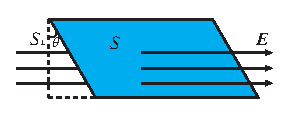
\includegraphics[scale=1.4]{C7-fig6.eps}
	\caption{电场线穿过曲面}
\end{figure}

\subsection{静电场高斯定理}

\begin{theorem}[静电场高斯定理]\label{C7-thgs}
	真空中任何静电场中, 穿过任一闭合曲线的电场强度通量, 数值上等于该闭合曲面包围电荷量的代数和乘$\dfrac{1}{\varepsilon_0}$, 即
	
	\begin{equation}
		\varPhi_e = \dfrac{1}{\varepsilon_0} \sum\limits_{S\text{内}} q_i \label{C7-eq4}
	\end{equation}
	
\end{theorem}

下面分几种情况证明其正确性. 

\begin{enumerate}
	\item 穿过包围点电荷$q$的任意闭合曲面$S$有
	
	\begin{equation}
		\varPhi_e = \dfrac{q}{\varepsilon_0} \label{C7-eq5}
	\end{equation}
	
	对于一个电荷量为$q$的点电荷, 其电场强度
	
	\begin{equation}
		\va*{E} = \dfrac{q}{4 \pi \varepsilon_0 r^2}\va*{e_r} \label{C7-eq6}
	\end{equation}
	
	若用一规则球壳包围它, 则
	
	\begin{equation}
		\varPhi_e = \int_{S}{\va*{E} \cdot \dd{\va*{S}}} = \dfrac{q \cdot 4 \pi r^2}{4 \pi \varepsilon_0 r^2} = \dfrac{q}{\varepsilon_0} \label{C7-eq7}
	\end{equation}
	
	这个球壳半径不影响结果, 用任意一个不规则曲面包围这个球壳也会有磁通量相同.
	
	\begin{figure}[h]
		\centering
		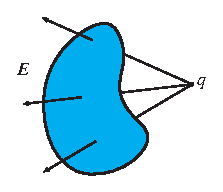
\includegraphics[scale=1.4]{C7-fig7.eps}
	\end{figure}
	
	\item 不包围电荷的高斯面的$\varPhi_e = 0$, 有多少电场线穿入就有多少电场线穿出, 故$\varPhi_e = 0$. 
	
	\vskip 0.3cm
	
	\item 详见课本P 253, $\displaystyle \oint_S E \cdot \dd{S} = \dfrac{1}{\varepsilon_0} \sum\limits_{i = 1} q_i$
	
\end{enumerate}

\begin{note}
	
	$\bullet$ 高斯定理中面元处的场强是该处的真实场强, 而非限定的其包围的电荷的场强. 
	
	$\bullet$ 高斯定理的有效应用还是有一定的限制, 实际上如果高斯面为不规则曲面, 使用高斯定理的意义不大. 其常用于求对称物体场强部分布. 
	
\end{note}

\newpage 

\begin{example}
	求均匀带正电球面内外场强, 球面电荷量为$Q$.
	
	\begin{figure}[h]
		\centering
		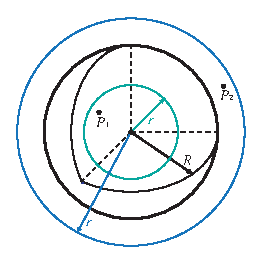
\includegraphics[scale=1.1]{C7-fig8.eps}
		\caption{均匀带正电球面}
	\end{figure}
	
	\begin{solution}
		设球面半径为$R$. 无论是球面内的$P_1$, 还是球面外的$P_2$, 均有场强方向沿着$\overrightarrow{OP_1}$或沿$\overrightarrow{OP_2}$方向, 所以作一半径为$r$的高斯球面, 其上任一点场强大小相同, 方向均沿半径方向, 所以
		
		\begin{align*}
			E &\perp S_{\bot} \\ 
			\varPhi_e &= 4 \pi r^2 E 
		\end{align*}
		
		对任意半径小于$R$的高斯球面均有
		
		\begin{equation*}
			\varPhi_e = \dfrac{1}{\varepsilon_0}\sum\limits_{i} q_i 
		\end{equation*}
	    
	    因为球面内无电荷, 所以电通量为0, 于是$E=0$, 球面内无电场分布. 
		
		当取高斯球面半径大于$R$时, 有$4\pi\varepsilon_0 r^2 E = Q$, 此时可得
		
		\begin{equation*}
			E = \dfrac{Q}{4\pi\varepsilon_0 r^2}
		\end{equation*}

		综上, 球面电场分布为
		
		\begin{equation*}
			E = \begin{cases}
				0, ~r &< R \\
				\dfrac{Q}{4\pi\varepsilon_0 r^2}, ~r &\geq R 
			\end{cases}
		\end{equation*}
		
		\begin{figure}[h]
			\centering
			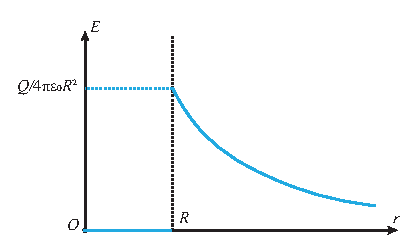
\includegraphics[scale=1.2]{C7-fig9.eps}
			\caption{场强分布示意}
			\label{C7-fig9}
		\end{figure}
		
	\end{solution}
	
\end{example}

\begin{example}
	对于均匀带电球体, 其半径为$R$, 电荷量为$Q$, 求其场强分布. 
	
	\begin{figure}[h]
		\centering
		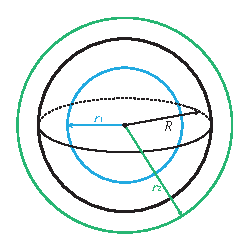
\includegraphics[scale=1.4]{C7-fig10.eps}
		\caption{均匀带电球体}
	\end{figure}
	
	\begin{solution}
		
		(1) 当高斯曲面选为半径小于$R$的均匀球面时有
		
		\begin{equation*}
			4\pi r_1^2 E = \dfrac{Q \cdot {{{\dfrac{4}{3}}\pi r_1^3}}}{{\dfrac{4}{3}}\pi R^3} = {\qty(\dfrac{r_1}{R})}^3 Q \Rightarrow E = \dfrac{Q r_1}{4\pi R^3} 
		\end{equation*}
	
	    (2) 当高斯曲面选为半径大于R的均匀球面时有
	    
	    \begin{equation*}
	    	4\pi r_2^2 E = \dfrac{Q}{\varepsilon_0} \Rightarrow E = \dfrac{Q}{4\pi\varepsilon_0 r_2^2}
	    \end{equation*}
	    
	    方向可由球体带电性质判断. 这个结果和地心引力以及重力加速度随离地心半径的关系一致. 
	    
	    \begin{figure}[h]
	    	\centering
	    	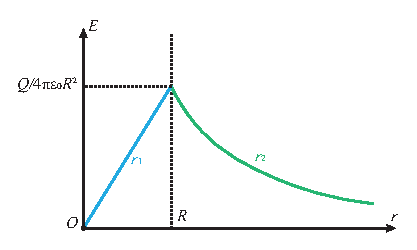
\includegraphics[scale=1.4]{C7-fig11.eps}
	    	\caption{场强分布示意}
	    \end{figure}
	    
	\end{solution}
	
\end{example}

\newpage

\begin{example}
	有一无限长均匀带电的圆柱面, 已知其横截面半径为$R$, 沿圆柱面轴线方向的电荷线密度为$\lambda$, 求圆柱面内外场强分布. 
	
	\begin{figure}[h]
		\centering
		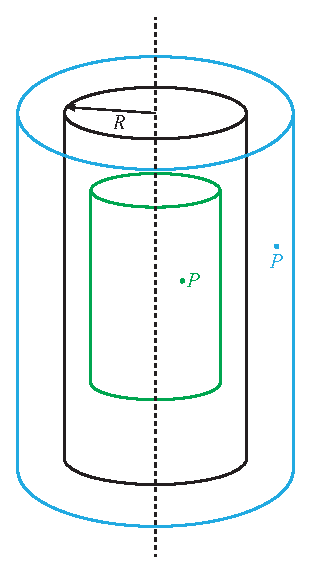
\includegraphics[scale=0.8]{C7-fig12.eps}
		\caption{无限长均匀带电的圆柱面}
	\end{figure}
	
	\begin{solution}
		
		对于空间上任一点$P$, $P$点场强在不沿半径方向相互抵消, 故场强沿半径方向, 仍有$\va*{E}\perp \va*{S}_{\bot}$. 
		
		取高斯面形状为圆柱形, 因为圆柱面无限长, 在距离中心轴距离相同的位置上场强大小相等所以不用考虑场强在沿轴线的变化情况. 所以$h$不影响求解. 
		
		当$r \leq R$时, 有
		
		\begin{equation*}
			2 \pi r h E = q
		\end{equation*}
		
		因为圆柱面内无电荷, 所以$E = 0$.
		
		当$r > R$时, 有
		
		\begin{equation*}
			2 \pi r h E = \dfrac{h \lambda}{\varepsilon_0} \Rightarrow E = \dfrac{\lambda}{2 \varepsilon_0 \pi r}
		\end{equation*}
		
		这里圆柱上下底面$\va*{E}\cdot \va*{S}_{\bot} = 0$, 故只有侧面有电通量. 
		
		综上所述, 
		
		\begin{equation*}
			E = \begin{cases}
				0, r \leq R \\
				\dfrac{\lambda}{2 \varepsilon_0 \pi r}, r > R
			\end{cases}
		\end{equation*}
		
	\end{solution}
	
\end{example}

\begin{note}
	
	请依此法尝试求解无限长均匀带电圆柱的场强分布. 同样还是场强方向只沿半径方向, 高斯面仍可取圆柱面且上下底面均无电通量. 
	
\end{note}

\newpage

\begin{example}
	均匀带电的无限大平面薄板, 电荷面密度为$\sigma$, 求场强分布. 
	
	\begin{figure}[h]
		\centering
		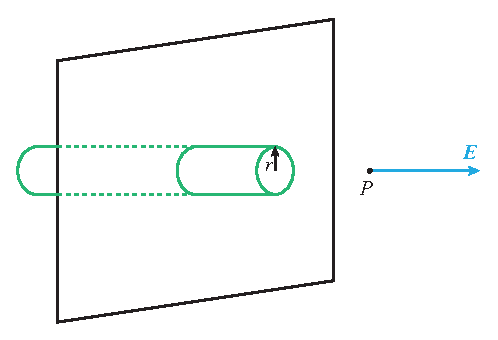
\includegraphics[scale=0.7]{C7-fig13.eps}
		\caption{均匀带电的无限大平面薄板}
	\end{figure}
	
	\begin{solution}
		由对称性, 任意位置的$P$点均有场强方向垂直平面. 取高斯面如图. 
		
		同样因为是无限大平面, $r$的大小不影响$E$的结果. 
		
		于是有
		
		\begin{equation*}
			2 \pi r^2 E = \dfrac{\sigma S}{\varepsilon_0} \Rightarrow E = \dfrac{\sigma}{2\varepsilon_0}
		\end{equation*}
		
		注意到$E$只与$\sigma$有关, 与$P$点到$O$平面的垂直距离无关. 
		
	\end{solution}
	
\end{example}

\begin{note}
	
	这个模型有两种变形: 
	
	(1) 把“薄板”改为有厚度的导体板, 此时取高斯面要取成一个底面在导体板内, 一个底面在导体板外的形式. 这样因为导体内无电场, 于是有
	
	\begin{figure}[h]
		\centering
		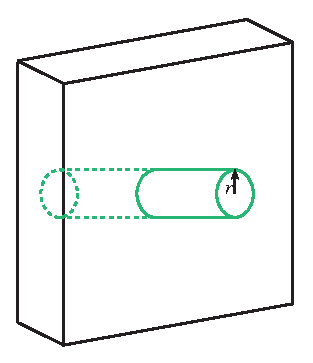
\includegraphics[scale=0.6]{C7-fig14.eps}
	\end{figure}
	
	\begin{equation*}
		\pi r^2 E = \dfrac{\pi r^2 \sigma}{\varepsilon_0} \Rightarrow E = \dfrac{\sigma}{\varepsilon_0}
	\end{equation*}
	
	后面会知道导体内无电荷分布, 电荷集中在“表面”. 
	
	(2) 把“一个”变成“两个”, 且这两个薄板带电荷量相反, 即
	
	\begin{figure}[H]
		\centering
		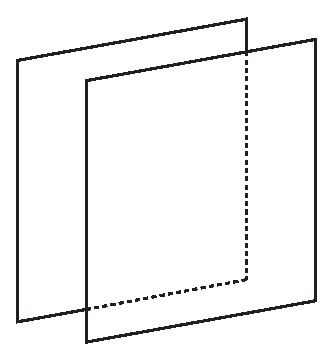
\includegraphics[scale=0.6]{C7-fig15.eps}
	\end{figure}
	
	此时分两步取高斯面. 
	
	第一步, 取
	
	\begin{figure}[H]
		\centering
		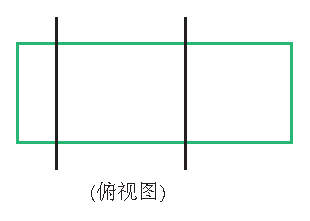
\includegraphics[scale=0.7]{C7-fig16.eps}
	\end{figure}
	
	可得$E = 0$, 即两板外$E = 0$. 
	
	第二步, 取
	
	\begin{figure}[H]
		\centering
		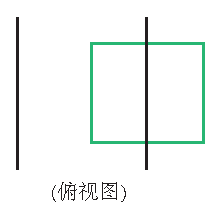
\includegraphics[scale=0.7]{C7-fig17.eps}
	\end{figure}
	
	可得两板间$E = \dfrac{\sigma}{\varepsilon_0}$
	
	这在后面电容器中有些作用. 
\end{note}

\subsection{环路定理}

高斯定理说明电场为有源场, 安培环路定理说明电场为保守力场. 

\textbf{静电力做功的特点}

\begin{figure}[H]
	\centering
	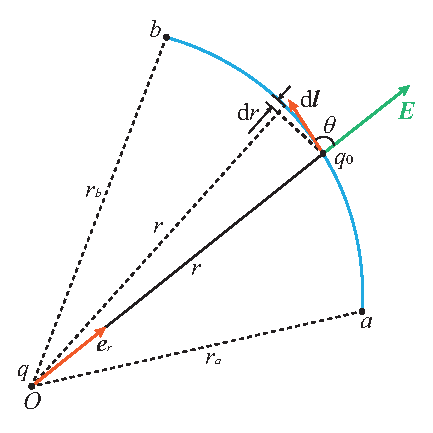
\includegraphics[scale=0.7]{C7-fig18.eps}
	\caption{静电力做功示意}
\end{figure}

假设$O$点有一个元电荷激发的电场, 一试验电荷从$a$到$b$运动, 则

\begin{equation}
	\dd{A} = \va*{F} \cdot \dd{\va*{l}} = q_0 \va*{E} \cdot \dd{\va*{l}} =  \dfrac{q_0 q}{4 \pi \varepsilon_0 r^2}\va*{e_r} \cdot \dd{\va*{l}} = \dfrac{q_0 q}{4 \pi \varepsilon_0 r^2} \cos \theta \dd{l} = \dfrac{q_0 q}{4 \pi \varepsilon_0 r^2} \dd{r} \label{C7-eq8}
\end{equation}

则从$a$到$b$电场总功

\begin{equation}
	A = \int_{a}^{b} \dd{A} = \int_{r_a}^{r_b} {\dfrac{q_0 q}{4 \pi \varepsilon_0 r^2} \dd{r}} = \dfrac{q_0 q}{4 \pi \varepsilon_0 r^2}(\dfrac{1}{r_a} - \dfrac{1}{r_b}) \label{C7-eq9}
\end{equation}

即单个电荷激发出的电场做功只与试验电荷与中心电荷的距离有关, 而与路径无关. 静电场与重力场一样是保守场. 

\begin{theorem}[静电场的环路定理]
	试验电荷从$a$经闭合路径$l_1$, $l_2$回到$a$, 在这个过程中电场力所做的功为
	
	\begin{figure}[H]
		\centering
		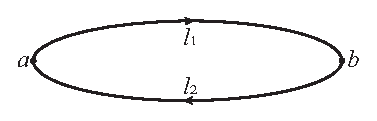
\includegraphics[scale=1.0]{C7-fig19.eps}
	\end{figure}
	
	\begin{equation}
		A = \oint_{L}{q_0 E \cdot \dd{l}} = 0 \label{C7-eq10}
	\end{equation}
	
	静电场场强沿任何闭合路径的线积分为零. 
\end{theorem}

\subsection{电势与电势能}

前面讲到静电场为保守场, 即做功只与电荷始末位置有关, 因此可引入势能$E_{\textrm{p}a}$, 即

\begin{equation}
	E_{\textrm{p}b} - E_{\textrm{p}a} = \int_{a}^{b}{\va*{E} \cdot q \cdot \dd{\va*{l}}} \Rightarrow \dfrac{E_{\textrm{p}b} - E_{\textrm{p}a}}{q}  = \int_{a}^{b}{\va*{E} \cdot \dd{\va*{l}}} \label{C7-eq11}
\end{equation}

式(\ref{C7-eq11})右侧与$q$无关, 不包含任何试验电荷量, 因此是电场的性质, 与电场强度异曲同工, 而左侧是势能变化量除以试验电荷量, 定义为从$a$到$b$过程中的电势差$U_{ab}$, 其中$\dfrac{E_{\textrm{p}b}}{q}$定义为$b$处电势$V_b$, $\dfrac{E_{\textrm{p}a}}{q}$定义为$a$处电势$V_a$. 它们满足

\begin{equation}
	U_{ab} = V_b - V_a
\end{equation}

可与高度和高度差类比. 

\textbf{电势的求解}

\begin{enumerate}[itemindent=1em]
	
	\item 从前面以单个点电荷形成的电场为条件推出的电势表达式来看
	\begin{equation}
		V_a = \dfrac{q_0}{4 \pi \varepsilon_0} \dfrac{1}{r_a} \label{C7-eq12}
	\end{equation}
	那么当$r_a \rightarrow +\infty$时$V_a = 0$, $V_a$相当于$U_{a +\infty}$, 即\textbf{某试验电荷在某点的电势能为从该点将该试验电荷移到无穷远处(零势能点)过程中电场所做功的大小}, 电势自然为电势能除以试验电荷量. 
	
	因此在求电势的时候即可使用$U_{a +\infty}$的思路, 先求电势能除以试验电荷量, 一般要用到电势叠加原理(这个方法常用于带电圆环产生的电场的电势计算), 由前定义 
	
	\begin{equation}
		V_p = \int_{p}^{+\infty}{\va*{E}\cdot \dd{\va*{l}}} \label{C7-eq13}
	\end{equation}
	
	因为电场强度服从矢量加和, 即
	
	\begin{equation}
		V_p = \int_{p}^{+\infty}{(\va*{E}_1 + \va*{E}_2 + \cdots + \va*{E}_n)} \dd{\va*{l}} = V_{1p} + V_{2p} + \cdots + V_{Np} = \sum\limits_{i=1}^{n}{V_{ip}} \label{C7-eq14}
	\end{equation}
	
	即某位置的电势为该位置在每一个单独场源电荷形成的电场中的电势之和
	
	\begin{equation}
		V_p = \dfrac{1}{4\pi\varepsilon_0}\sum\limits_{i=1}^{n}\dfrac{q_i}{r_i}
	\end{equation}

	电势是标量, 因此在求电势的积分时不需分解, 比较方便. 
	
	\item 对于用积分不太方便, 比如均匀带电的球体就可先用高斯定理求出$\va*{E}$沿半径的分布, 再用
	
	\begin{equation*}
		V_p = \int_{p}^{+\infty}{\va*{E}\cdot \dd{\va*{l}}}
	\end{equation*}
	
	积分求解. 
	
\end{enumerate}

\begin{example}
	(应用方法一) 电荷密度$\lambda$均匀分布在半径为$R$的圆环上, 计算$P$点电势. 
	
	\begin{figure}[H]
		\centering
		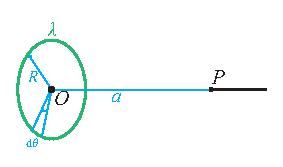
\includegraphics[scale=1.2]{C7-fig20.eps}
		\caption{均匀带电细圆环}
	\end{figure}
	
	\begin{solution}
		
		取一段小圆弧, 其电量为$\lambda R \dd{\theta}$, 它在$P$点电势为
		
		\begin{equation*}
			\dfrac{1}{4\pi\varepsilon_0}\int\dfrac{\lambda R \dd{\theta}}{\sqrt{R^2 + a^2}}
		\end{equation*}
		
		由电势叠加
		
		\begin{equation*}
			V_p = \dfrac{\lambda R}{4\pi\varepsilon_0\sqrt{R^2+a^2}}\int_{0}^{2\pi}\dd{\theta} = \dfrac{2\pi\lambda R}{4\pi\varepsilon_0\sqrt{R^2+a^2}} = \dfrac{Q}{4\pi\varepsilon_0\sqrt{R^2+a^2}}
		\end{equation*}
		
	\end{solution}
	
\end{example}

\begin{example}
	(应用方法二) 半径为$R$的电荷总量为$Q$的均匀带电球面内外电势分布. 
	
	\begin{figure}[H]
		\centering
		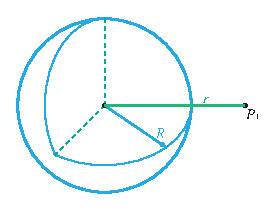
\includegraphics[scale=1.2]{C7-fig21.eps}
		\caption{均匀带电球面}
	\end{figure}
	
	\begin{solution}
		
		因为电场分布对称, 先用高斯定理求E分布(当然也可以用前面介绍的积分求场强的方法). 
		
		由图(\ref{C7-fig9})可知球面内无场强, $E = 0$, 故不存在电势升降. 球面与球面内等势, 均等于球面电势, 即
		
		当$r \leq R$时
		
		\begin{equation*}
			V_R = V_r = \int_{R}^{+\infty}{\dfrac{Q}{4\pi\varepsilon_0 r^2}\dd{r}} = \dfrac{Q}{4\pi\varepsilon_0 R} 
		\end{equation*}
		
		当$r > R$时 
		
		\begin{equation*}
			V_r = \int_{r}^{+\infty}{\dfrac{Q}{4\pi\varepsilon_0 r^2}\dd{r}} = \dfrac{Q}{4\pi\varepsilon_0 r}
		\end{equation*}
		
		故电势分布情况如下
		
		\begin{figure}[H]
			\centering
			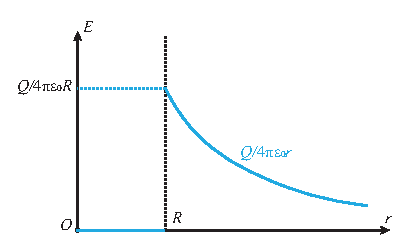
\includegraphics[scale=1.2]{C7-fig22.eps}
		\end{figure}
		
	\end{solution}
	
\end{example}

\begin{example}
	(应用两种方法均可) 半径分别为$R_A$, $R_B$的两个同心均匀带电球面, 所带电荷为$Q_A$, $Q_B$, 求两球面电势. 
	
	\begin{figure}[H]
		\centering
		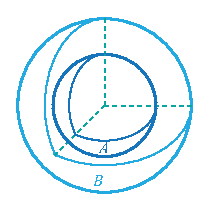
\includegraphics[scale=1.2]{C7-fig23.eps}
		\caption{均匀带电同心球面}
	\end{figure}
	
	\begin{solution}
		
		$V_A$ = $A$球在$A$表面电势 + $B$球在$A$表面电势 = $A$球在$A$表面电势 + $B$球在$B$表面电势 
		
		因为$B$球面内无电场, 所以$B$球等势. 
		$V_B$ = $A$球在$B$球表面电势 + $B$球在$B$表面电势 (电势叠加原理)
		
		具体求法参考方法二. 
	\end{solution}
	
\end{example}

\section{静电场中的导体} \label{7.3}

\subsection{导体静电平衡}

在外加电场的条件下, 因为金属导体中的电子是游离的, 因此电子会沿电场反方向移动, 在导体的一端积累负电荷, 因为系统电荷守恒, 所以另一端会自然的积累正电子, 从而产生感应电场且感应电场与外加电场方向相反, 当两者大小相等时, 导体内电子不再移动, 从而达到平衡. 

\begin{figure}[H]
	\centering
	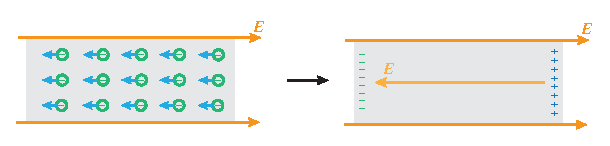
\includegraphics[scale=1.4]{C7-fig24.eps}
	\caption{导体静电平衡}
\end{figure}

导体静电平衡特点与要求: 

\begin{enumerate}[itemindent=1em]
	
	\item 导体内部场强为0; 
	\item 导体表面外电场强度方向垂直导体表面(否则会有电荷移动)且满足$E = \dfrac{\sigma}{\varepsilon_0}$(前面在用高斯定理推导场强时已介绍, 这里把导体表面取微元近似看成平面即可); 
	\item 电荷只分布在导体表面; 
	\item 整个导体是等势体. 
	
\end{enumerate}

\subsection{静电屏蔽}

这一部分最好不要记模型, 应该结合高斯定理, 静电平衡的特点来推出电荷分布情况, 否则容易混乱, 最重要的题型就是求电荷分布. 
\begin{example}
	不带电空腔且内无带电体, 在外部电场作用下电荷分布.
	
	\begin{figure}[H]
		\centering
		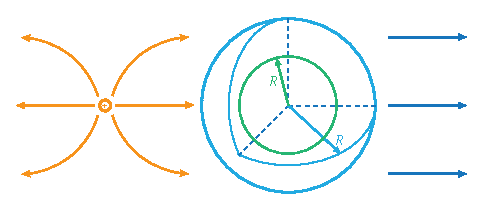
\includegraphics[scale=1.5]{C7-fig25.eps}
		\caption{不带电空腔且内无带电体}
		\label{C7-fig25}
	\end{figure}
	
	\begin{solution}
		
		重要的有两件事: 第一, 空腔内表面有没有电荷; 第二, 空腔外表面电荷哪边为正. 
		
		从静电平衡条件, 静电平衡导体等势, 空腔内无电场, 做一包含$R$的高斯面$r$, $\varPhi_e = 0$, 则$\sum q = 0$, 且因为内等势, 无电场, 电荷分布均匀. 
		
		还是内无场强, 外部电场有向右场强, 易知外表面电荷分布如图(\ref{C7-fig25}), 且左右电荷量相等.
	\end{solution}
	
\end{example}

\newpage

\begin{example}
	空腔不带电, 内部含带电体. 
	
	\begin{figure}[H]
		\centering
		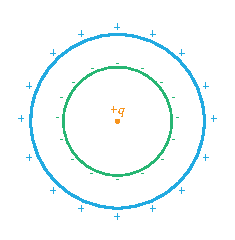
\includegraphics[scale=1.4]{C7-fig26.eps}
		\caption{不带电空腔且内含带电体}
	\end{figure}
	
	\begin{solution}
		
		同样是内外表面有无电荷, 如何分布两个关键问题. 
		
		高斯定理可知内表面带电$-q$, 电荷守恒可知外表面带电$+q$. 
		
		如果把外壳接地, 高斯定理仍得内表面带电$-q$, 此时外表面正电流向大地为0. \textbf{把握住高斯定理, 电荷守恒即可.}\footnote{思考: 内表面接地如何? }
		
	\end{solution}
\end{example}

静电屏蔽是指外加的电场不会影响导体空腔内的物体, 也指空腔外表面接地后内部电场对外无影响. 

\begin{example}
	两平行且面积相等导体板, 认为无限大(面积$S~\gg$板间距$d$). 已知$q_A$, $q_B$, 求静电平衡时各表面电荷面密度. 
	
	\begin{figure}[H]
		\centering
		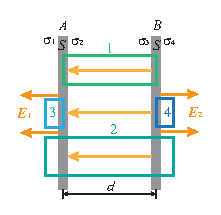
\includegraphics[scale=1.5]{C7-fig27.eps}
		\caption{平行且面积相等导体板}
	\end{figure}
	
	\begin{solution}
		设$\sigma_1$, $\sigma_2$, $\sigma_3$, $\sigma_4$分别为各表面电荷面密度.
		
		取高斯面1知
		
		\begin{equation*}
			\sigma_2 S + \sigma_3 S = 0 \Rightarrow \sigma_2 = -\sigma_3
		\end{equation*}
		
		取高斯面2知
		
		\begin{equation*}
			\dfrac{\sigma_1 S + \sigma_2 S + \sigma_3 S + \sigma_4 S}{\varepsilon_0} = E_1 S - E_2 S \Rightarrow \sigma_1 + \sigma_2 + \sigma_3 + \sigma_4 = E_1 - E_2
		\end{equation*}
		
		取高斯面3, 4知
		
		\begin{equation*}
			\begin{cases}
				\dfrac{\sigma_1 S}{\varepsilon_0} = E_1 S \\   \dfrac{\sigma_4 S}{\varepsilon_0} = E_2 S 
			\end{cases} 
		    \Rightarrow
		    \begin{cases}
		    	\dfrac{\sigma_1}{\varepsilon_0} = E_1 \\  \dfrac{\sigma_4}{\varepsilon_0} = E_2
		    \end{cases}
		\end{equation*}

		最后根据电荷守恒有
		
		\begin{align*}
			\sigma_1 S + \sigma_2 S &= q_1 \\ 
			\sigma_3 S + \sigma_4 S &= q_2 
		\end{align*}
		
		综上解得
		
		\begin{align*}
			\sigma_1 &= \sigma_4 = \dfrac{q_A + q_B}{2 S} \\
			\sigma_2 &= -\sigma_3 = \dfrac{q_A-q_B}{2S}
		\end{align*}
		
	\end{solution}
	
\end{example}

\section{各向同性电介质} \label{7.4}

导体讲完讲电介质, 这一部分主要讲各向同性电介质. 

\subsection{电介质极化}

1. 自身有电偶极矩的电介质的极化

这种电介质分子正负电荷中心不重合(就像纯水), 这种电介质分子在外电场作用下会有规则排列此时内部会出现“$\leftarrow$”与外电场反方向的电场, 削弱外电场.

\textbf{此时极化出的电荷是与自由电荷不同的, 称极化电荷, 它不能“流动”.} 

\begin{figure}[H]
	\centering
	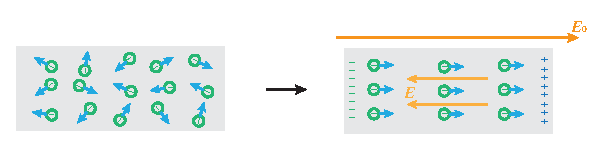
\includegraphics[scale=1.4]{C7-fig28.eps}
\end{figure}

2. 自身无电偶极矩的电介质
这种电介质分子正负电荷中心重合, 在外电场作用时正负电荷中心分离, 也表现为削弱外电场. 

极化特点: 与导体不同, 极化只会削弱外电场而不会抵消外电场, 削弱后的电场强度为$E = \dfrac{E_0}{\varepsilon_r}$, 其中$\varepsilon_r$为电介质的相对介电常数.

\subsection{介质中的高斯定理和电位移矢量}

强调一下, \textbf{真空中高斯定理}的内容见定理(\ref{C7-thgs}). 

下面推导电介质中的高斯定理. 

两个有厚度的极板间充入电介质, 其相对介电常数为$\varepsilon_r$, 因为极化, 极板附近有相反极化电荷. 

\begin{figure}[H]
	\centering
	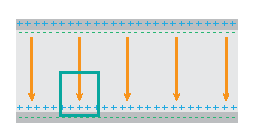
\includegraphics[scale=1.4]{C7-fig29.eps}
\end{figure}

\begin{align*}
	&\text{无极化时:~}E = \dfrac{\sigma_0}{\varepsilon_r} \\
	&\text{有极化时:~}\dfrac{E}{\varepsilon_0} = \dfrac{\sigma_0 - \sigma'}{\varepsilon_0}\text{(这里包含自由电荷与极化电荷)}
\end{align*}

所以

\begin{equation}
	\sigma'= \qty(1 - \dfrac{1}{\varepsilon_r}) \sigma_0 \text{(极化电荷)}
	\label{C7-eq15}
\end{equation}

代入高斯定理

\begin{equation}
	\oint_{S}{\va*{E} \cdot \dd{\va*{S}}} = \dfrac{1}{\varepsilon_0}(\sigma_0 - \sigma') \Delta S = \dfrac{1}{\sigma_0}(1 - 1 + \dfrac{1}{\varepsilon_r})\cdot \sigma_0 \Delta S = \dfrac{\sigma_0 \Delta S}{\varepsilon_0 \varepsilon_r}
	\label{C7-eq16}
\end{equation}

所以

\begin{equation}
	\oint_{S}{E\varepsilon_0\varepsilon_r\dd{S}} = \sigma_0 \Delta S = q \label{C7-eq17}
\end{equation}

亦可写成

\begin{equation}
	\oint_{S}{E\varepsilon_r \dd{S}} = \dfrac{q}{\varepsilon_0} \label{C7-eq18}
\end{equation}

这样在形式上与真空中高斯定理一致, 这就是介质中高斯定理, 其内容为: 通过任意闭合曲面的电位移矢量等于该闭合曲面所包围的自由电荷代数和. 

为了方便记忆(与真空中的高斯定理统一), 可以统一记成

\begin{equation}
	\oint_{S}{\va*{E}\cdot \dd{\va*{S}}} = \dfrac{q}{\varepsilon} \label{C7-eq19}
\end{equation}

其中, $\varepsilon$是介电常数, 真空介电常数为$\varepsilon_0$, 即原本用的高斯定理, 而介质中为$\varepsilon_0\varepsilon_r$, 也就是介质中高斯定理. 

电位移矢量$\va*{D}$是$\va*{E}\varepsilon_0\varepsilon_r$, 即$\int_{S}{\vec{D}\cdot \dd{\va*{S}}} = q$, 是用介质中高斯定理定义的. 

\subsection{电容器}

只用记一个定义

\begin{equation}
	C = \dfrac{Q}{U} \label{C7-eq20}
\end{equation}

对于孤立导体, 可以认为是导体与无穷远构成一个电容器, $U$为导体电势; 对于正常电容器, $Q$为电容器电量, $U$为两极板电势差(通常带等量电量). 

$U$对于电容器的题目来说基本是用对场强积分得来, 即

\begin{equation}
	U = \int_{a}^{b} \va*{E} \dd{x} \label{C7-eq21}
\end{equation}

而$E$可用介质中高斯定理求(因为电容器间常加电介质).

\begin{example}
	$A$, $B$两极板面积均为$S$, 电荷量相反. 两板间充入相对介电常数$\varepsilon_r$的电介质, 求电容$C$.
	
	\begin{figure}[H]
		\centering
		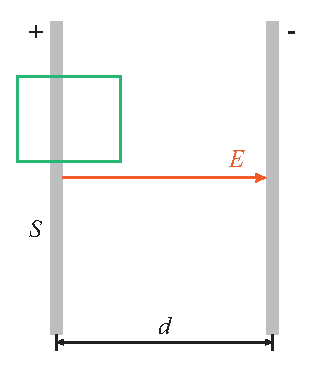
\includegraphics[scale=0.8]{C7-fig30.eps}
	\end{figure}
	
	\begin{solution}
		
		由介质中高斯定理
		
		\begin{equation*}
			E \cdot \dd{S} = \dfrac{\sigma \dd{S}}{\varepsilon_0\varepsilon_r} \Rightarrow E = \dfrac{\sigma}{\varepsilon_0\varepsilon_r}
		\end{equation*}
		
		则
		
		\begin{equation*}
			\Delta U = Ed = \dfrac{\sigma d}{\varepsilon_0 \varepsilon_r}
		\end{equation*}
	
	    于是
		
		\begin{equation*}
			C = Q \Delta U = \dfrac{\sigma S}{\dfrac{\sigma d}{\varepsilon_0 \varepsilon_r}} = \dfrac{\varepsilon_0 \varepsilon_r S}{d}
		\end{equation*}
		
		其它形状电容器同理. 
		
	\end{solution}
	
\end{example}

电容器的串联并联与弹簧串联并联规律一致, 与电阻串联并联规律相反. 

\section{静电场的能量}

\subsection{点电荷系的电势能} \label{7.5}

初始时$q_1$, $q_2$均位于无穷远处, 无论先把$q_1$移到$q_1'$再移$q_2$到$q_2'$还是先移$q_2$到$q_2'$再移$q_1$到$q_1'$均有系统势能

\begin{equation}
	W_2 = \dfrac{q_1 q_2}{4 \pi \varepsilon_0 r} = \dfrac{1}{2}q_1 V_1 + \dfrac{1}{2}q_2 V_2 \label{C7-eq22}
\end{equation}

如果扩展到三个点电荷仍有系统的电势能为

\begin{equation}
	W_3 = \dfrac{1}{2}q_1 V_1 + \dfrac{1}{2}q_1 V_1 + \dfrac{1}{2}q_3 V_3
\end{equation}

对$n$个质点系也有此规律, 即

\begin{equation}
	W = \dfrac{1}{2} \sum\limits_{i=1}^{n}{q_i V_i} \label{C7-eq23}
\end{equation}

$V_i$为此点电荷在其他点电荷的电场中的电势. 

\subsection{电荷连续分布的带电体自能}

\begin{equation}
	W = \dfrac{1}{2} \int_{V} V \dd{q} \label{C7-eq24}
\end{equation}

和点电荷系公式一样, 只是要积分. 

\subsection{电容器的电势能}

电容器充电时就在储能, 电源对电荷做的功就是储存的电势能. 

\begin{equation}
	\dd{A} = U_q \dd{q} = \dfrac{q}{c} \dd{q} \Rightarrow A=\frac{Q^2}{2C} \label{C7-eq25}
\end{equation}

又因为$Q = CU$, 所以

\begin{equation}
	W = \dfrac{Q^2}{2C} = \dfrac{C U^2}{2} = \dfrac{QU}{2} \label{C7-eq26}
\end{equation}

\subsection{静电场的能量}

\begin{equation}
	W_e = \dfrac{1}{2} \va*{D} \cdot \va*{E} \label{C7-eq27}
\end{equation}

其中, $\va*{D} = \va*{E}\varepsilon_0\varepsilon_r$. 这是任何带电体产生的电场的能量密度. 

无论是否均匀, 均有总静电能

\begin{equation}
	W = \int_{V}{\dfrac{1}{2}\va*{D}\cdot\va*{E} \dd{V}} \label{C7-eq28}
\end{equation}
